\lecture{Nov. 1}

\begin{thm}[Unique Prime Factorization]
    Every integer $n\geq 2$ can be expressed uniquely in the form \[n=\prod_{i=1}^l p_i = p_1p_2\cdots p_l\] for some $l\in\mathbb{Z}^+$ and some primes $p_1,p_2,\cdots,p_l$ with $p_1\leq p_2\leq \cdots \leq p_l$.
\end{thm}

\begin{proof}
    First we show existence. Let $n\geq 2$. Suppose, inductively, that every integer $k$ with $2\leq k < n$ can be written (uniquely) in the required form. If $n$ is prime then $n = p_1$ with $p_1 = n$.
    
    Suppose $n$ is composite, say $n=ab$ with $1<a<n$ and $1<b<n$. Since $2\leq a < n$ and $2\leq n < n$ we can write \[a = \prod_{i=1}^l p_i\] and \[b = \prod_{j=1}^m q_j\] with $l,m\in\mathbb{Z}$ and the $q_j,p_i$ are primes.
    
    Thus \begin{align*}
        n = & ab \\
        = & p_1p_2\cdots p_lq_1q_2\cdots q_m\\
        = & r_1r_2\cdots r_{l+m}
    \end{align*}
    
    where the $(l+m)-$tuple $(r_1,r_2,\cdots ,r_{l+m})$ is obtained by rearranging the entries of the \[\text{(l+m)-tuple } (p_1,p_2,\cdots ,p_{l},q_1,q_2,\cdots ,q_{m})\] into non-decreasing order.
    
    Next we prove uniqueness. We need to show that if $n=p_1p_2\cdots p_l$ and $n=q_1q_2\cdots q_m$ where $l,m\in\mathbb{Z}^+$ and the $p_i$ and $q_j$ are primes with $p_1\leq p_2 \leq \cdots \leq p_l$ and $q_1\leq q_2\leq \cdots q_m$, then $l=m$ and $p_i=q_i$ for all $i$.
    
    Suppose $n=p_1p_2\cdots p_l=q_1q_2\cdots q_m$ as above. Since $n=p_1p_2\cdots p_l$ we have $p_1\mid n$. Since $n=q_1q_2\cdots q_m$ we have $p_1\mid q_1q_2\cdots q_m$. It follows that $p_1\mid q_k$ for some $k$ with $1\leq k\leq m$. Say $p_1\mid q_k$. Since $q_k$ is prime, its only positive divisors are $1$ and $q_k$. Since $p_1\neq 1$, so $p_1 = q_k$. Similarly, $q_1 = p_j$ for some $j$ with $1\leq j\leq l$. Since $p_1 = q_k \geq q_1 = p_j \geq p_1$, so we must have $p_1=p_j=q_1$.
    
    Since $p_1p_2\cdots p_l = q_1q_2\cdots q_m$ and $q_1 = p_1 \neq 0$, we have $p_2p_3\cdots p_l = q_2q_3\cdots q_m$. A similar argument shows that $p_2 = q_2$. 
    
    Suppose for a contradiction, that $l\neq m$, say $l<m$. By repeating the above argument, we eventually obtain \[p_l = q_l \cdots q_m\] then $p_l = q_l$ then $1 = q_{l+1} \cdots q_m$. But each $q_j \geq 2$ so $q_{l+1} \cdots q_m \geq 2$, so we have a desired contradiction, hence $m=l$.
    
    Thus repeating the above argument gives \[p_1=q_1, p_2=q_2, \cdots ,p_l = q_l = q_m. \qedhere\] 
\end{proof}


\begin{defn}[Diophantine Equation]
    A Diophantine Equation is a polynomial equation where the variables represent integers.
\end{defn}

\begin{exmp}
    Solve \[x^2+y^2 = 25\]
\end{exmp}


\begin{center}
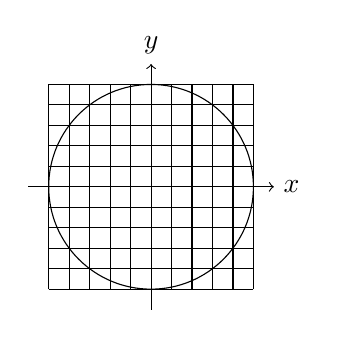
\begin{tikzpicture}[scale=0.26]
      \draw[->] (-6,0) -- (6,0) node[right] {$x$};
      \draw[->] (0,-6) -- (0,6) node[above] {$y$};
      \draw[-] (1,-5) -- (1,5);
      \draw[-] (2,-5) -- (2,5);
      \draw[-] (3,-5) -- (3,5);
      \draw[-] (4,-5) -- (4,5);
      \draw[-] (5,-5) -- (5,5);
      \draw[-] (-1,-5) -- (-1,5);
      \draw[-] (-2,-5) -- (-2,5);
      \draw[-] (-3,-5) -- (-3,5);
      \draw[-] (-4,-5) -- (-4,5);
      \draw[-] (-5,-5) -- (-5,5);
      \draw[-] (-5,-5) -- (5,-5);
      \draw[-] (-5,-4) -- (5,-4);
      \draw[-] (-5,-3) -- (5,-3);
      \draw[-] (-5,-2) -- (5,-2);
      \draw[-] (-5,-1) -- (5,-1);
      \draw[-] (-5,1) -- (5,1);
      \draw[-] (-5,2) -- (5,2);
      \draw[-] (-5,3) -- (5,3);
      \draw[-] (-5,4) -- (5,4);
      \draw[-] (-5,5) -- (5,5);
      \draw[] (0,0) circle (5);
\end{tikzpicture}
\end{center}


\begin{exmp}
    Solve \[x^2+y^2 = n\] in $\mathbb{Z}[i]$ where $i^2 = -1$
\end{exmp}

\begin{exmp}
    A Linear Diophantine Equation is an equation of the form \[ax+by = c\] where $a,b,c\in\mathbb{Z}$ with $(a,b)\neq 0$
\end{exmp}

\begin{exmp}[Pell's Equation]
    Solve \[x^2-dy^2 =\pm 1\]
\end{exmp}


\begin{exmp}[Pythagorean Triples]
    Solve \[x^2+y^2 = z^2\] \[x^2+y^2+z^2=w^2\]
\end{exmp}

\topic{Stereographic Projection}

\begin{center}
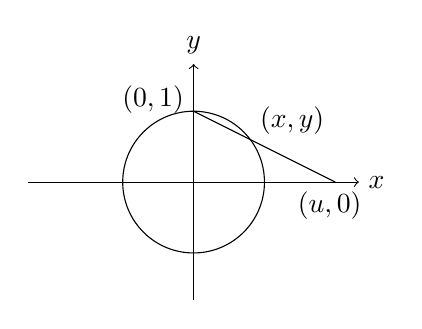
\begin{tikzpicture}[scale=0.3]
      \draw[->] (-7,0) -- (7,0) node[right] {$x$};
      \draw[->] (0,-5) -- (0,5) node[above] {$y$};
      \draw[] (0,0) circle (3);
      \draw[-] (0,3) -- (6,0);
      \filldraw[black] (0,3.5) circle (0pt) node[anchor=east] {$(0,1)$};
      \filldraw[black] (4,-1) circle (0pt) node[anchor=west] {$(u,0)$};
      \filldraw[black] (2.4,2.6) circle (0pt) node[anchor=west] {$(x,y)$}; 
\end{tikzpicture}
\end{center}